\documentclass{beamer}\usepackage[]{graphicx}\usepackage[]{xcolor}
% maxwidth is the original width if it is less than linewidth
% otherwise use linewidth (to make sure the graphics do not exceed the margin)
\makeatletter
\def\maxwidth{ %
  \ifdim\Gin@nat@width>\linewidth
    \linewidth
  \else
    \Gin@nat@width
  \fi
}
\makeatother

\definecolor{fgcolor}{rgb}{0.345, 0.345, 0.345}
\newcommand{\hlnum}[1]{\textcolor[rgb]{0.686,0.059,0.569}{#1}}%
\newcommand{\hlsng}[1]{\textcolor[rgb]{0.192,0.494,0.8}{#1}}%
\newcommand{\hlcom}[1]{\textcolor[rgb]{0.678,0.584,0.686}{\textit{#1}}}%
\newcommand{\hlopt}[1]{\textcolor[rgb]{0,0,0}{#1}}%
\newcommand{\hldef}[1]{\textcolor[rgb]{0.345,0.345,0.345}{#1}}%
\newcommand{\hlkwa}[1]{\textcolor[rgb]{0.161,0.373,0.58}{\textbf{#1}}}%
\newcommand{\hlkwb}[1]{\textcolor[rgb]{0.69,0.353,0.396}{#1}}%
\newcommand{\hlkwc}[1]{\textcolor[rgb]{0.333,0.667,0.333}{#1}}%
\newcommand{\hlkwd}[1]{\textcolor[rgb]{0.737,0.353,0.396}{\textbf{#1}}}%
\let\hlipl\hlkwb

\usepackage{framed}
\makeatletter
\newenvironment{kframe}{%
 \def\at@end@of@kframe{}%
 \ifinner\ifhmode%
  \def\at@end@of@kframe{\end{minipage}}%
  \begin{minipage}{\columnwidth}%
 \fi\fi%
 \def\FrameCommand##1{\hskip\@totalleftmargin \hskip-\fboxsep
 \colorbox{shadecolor}{##1}\hskip-\fboxsep
     % There is no \\@totalrightmargin, so:
     \hskip-\linewidth \hskip-\@totalleftmargin \hskip\columnwidth}%
 \MakeFramed {\advance\hsize-\width
   \@totalleftmargin\z@ \linewidth\hsize
   \@setminipage}}%
 {\par\unskip\endMakeFramed%
 \at@end@of@kframe}
\makeatother

\definecolor{shadecolor}{rgb}{.97, .97, .97}
\definecolor{messagecolor}{rgb}{0, 0, 0}
\definecolor{warningcolor}{rgb}{1, 0, 1}
\definecolor{errorcolor}{rgb}{1, 0, 0}
\newenvironment{knitrout}{}{} % an empty environment to be redefined in TeX

\usepackage{alltt}
\usetheme{Madrid}

% Adjust margins globally
\setbeamersize{text margin left=5mm, text margin right=5mm}

% Include logo in title page
\title[Travelers University Modeling Competition]{2024 Travelers University Modeling Competition: \\ CloverShield Insurance Company Modeling Problem}
\subtitle{LightGBM Modeling Approach}
\author[O.F. Fasanya]{Oluwafunmibi Omotayo Fasanya,}
\date{December 5, 2024}
% Add logos side by side
\titlegraphic{
    \begin{minipage}{0.45\textwidth}
        \centering
        
\includegraphics[width=5cm]{Travelers.jpeg}
    \end{minipage}%
    \hspace{-1.5cm}% Adjust spacing between logos
    \begin{minipage}{0.45\textwidth}
        \centering
        
\includegraphics[width=2cm]{nebraska-n.jpg} 
    \end{minipage}
}
\IfFileExists{upquote.sty}{\usepackage{upquote}}{}
\begin{document}


\frame{\titlepage}

% Section: Introduction
\section{Introduction}

\begin{frame}{Problem Statement}
\textbf{Objective:}
\begin{itemize}
    \item Develop a predictive model to forecast policyholder call frequency (\textit{call\_counts}) for CloverShield Insurance, based on customer and policy data.
\end{itemize}

\textbf{Goal:}
\begin{itemize}
    \item Reduce call center costs by optimizing resource allocation and improving efficiency through customer segmentation.
\end{itemize}

\textbf{Dataset:}
\begin{itemize}
    \item The training data has 21 columns with 80,000 rows while the test dataset has 20 columns (No “Call Counts” column) with 20,000 rows.
\end{itemize}
\end{frame}

\begin{frame}{Missing Values}
\textbf{Approach:}
\begin{itemize}
    \item Converted the values (-20, -2) to NA in the following columns:
    \begin{itemize}
        \item Age of the newest vehicle insured on a policy (\texttt{newest\_veh\_age})
        \item Telematic indicator (\texttt{telematics\_ind})
        \item Email delivery of documents (\texttt{pol\_edeliv\_ind})
    \end{itemize}
    \item Applied the same process to both the test and training datasets.
\end{itemize}

\begin{center}
    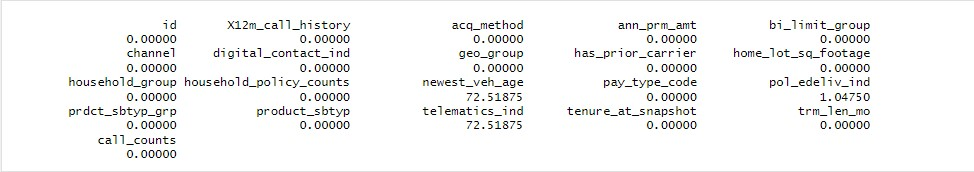
\includegraphics[width=0.8\textwidth]{Missing.jpg}
    \vspace{0.2cm} % Adjust spacing if necessary
    
    \footnotesize{Percentage of missing variable in Train Data.}
\end{center}
\end{frame}

% Section: Variable Selection
\section{Variable Selection}

\begin{frame}{Variable Selection}
\textbf{Handling Missing Values:}
\begin{itemize}
    \item Identified variables with high percentages of missing values and flagged them for imputation.
    \item Created missing value indicator variables to capture potential predictive information from missingness
    \item Imputation of Missing Values:
    \begin{itemize}
      \item Continuous variables: Median imputation (Robust to outliers).
      \item Categorical variables: Mode imputation (Most likely category).
    \end{itemize}
\end{itemize}
\end{frame}

\begin{frame}{Variable Selection}
\textbf{Correlation Analysis:}
\begin{itemize}
    \item Evaluated relationships with the target variable (\textit{call\_counts}):
    \begin{itemize}
        \item \textbf{Continuous variables:} Pearson correlation coefficient.
        \item \textbf{Categorical variables:} Point-Biserial Correlation to assess the relationship between binary predictors and           \textit{call\_counts}.
    \end{itemize}
    
    \item \textit{X12m\_call\_history} showed the highest positive correlation (0.28) with \textit{call\_counts} among continuous variables.
    \begin{center}
    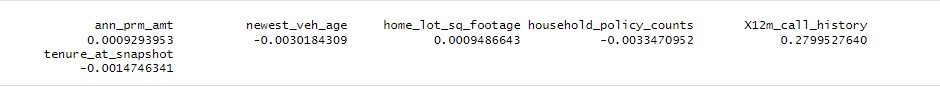
\includegraphics[width=0.8\textwidth]{AssC.jpg}
    \vspace{0.2cm} % Adjust spacing if necessary
    
    \footnotesize{Asscoiation between the continuous variables and call count}
\end{center}
    \item All of the categorical explanatory variable have very weak associations with call count.
\end{itemize}

\end{frame}

\begin{frame}{Variable Selection}
\textbf{Multicollinearity Check:}
\vspace{-0.2cm}
\begin{center}
    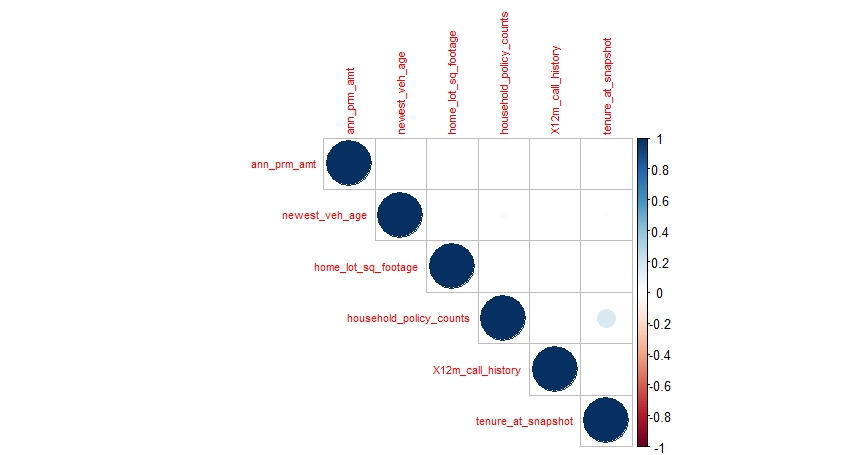
\includegraphics[width=0.7\textwidth]{Rplot1.jpeg}
    \vspace{0.2cm} % Adjust spacing if necessary
    
    \footnotesize{Correlation analysis between the continuous explanatory variables.}
\end{center}

\textbf{Categorical Encoding:}
\begin{itemize}
    \item Transformed categorical variables using one-hot encoding (dummy variables) to ensure compatibility with proposed model (LightGBM).
\end{itemize}

\end{frame}

\begin{frame}{Response Variable Summary}
\textbf{Key Insights:}
\begin{itemize}
    \item \textbf{Response Variable:} \texttt{call\_counts}
    \begin{itemize}
        \item Represents the count of calls for each customer.
    \end{itemize}
    \item \textbf{Percentage of Zero Values:}
    \begin{itemize}
        \item Approximately 50.18\% of customers have zero call counts in the training dataset.
    \end{itemize}
\end{itemize}

\begin{center}
    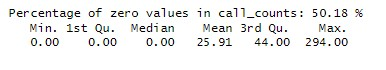
\includegraphics[width=0.7\textwidth]{Response.jpg}
\end{center}

\textbf{Distribution indicates potential sparsity in the response variable.}
\end{frame}


% Section: Methods Considered
\section{Methods Considered}

\begin{frame}{Methods Considered}
\textbf{Tree-Based Models:}
\begin{itemize}
    \item \textbf{Random Forest:} Captures non-linear relationships and interactions robustly.
    \item \textbf{XGBoost:} Effective gradient boosting algorithm for structured data.
    \item \textbf{Light Gradient Boosting Machine(LightGBM):} Efficient histogram-based decision tree with lower memory consumption.
\end{itemize}

\textbf{Zero-Inflated Models:}
\begin{itemize}
    \item \textbf{Zero-Inflated Poisson (ZIP):} Addresses excess zeros in count data.
    \item \textbf{Zero-Inflated Negative Binomial (ZINB):} Handles overdispersion and excess zeros.
    \item \textbf{Hurdle Model:} A two-part model designed to separately handle the zero and non-zero counts
\end{itemize}
\end{frame}

% Section: Chosen Method
\section{Chosen Method}

% Slide 1: Introduction to LightGBM
\begin{frame}{Chosen Method: LightGBM}
LightGBM is a gradient-boosting framework that integrates decision trees (weak learners) sequentially using boosting.
\begin{itemize}
    \item Boosting is an ensemble learning that trains weak learners iteratively on the dataset and combines them to form a strong learner
\end{itemize}
\begin{center}
    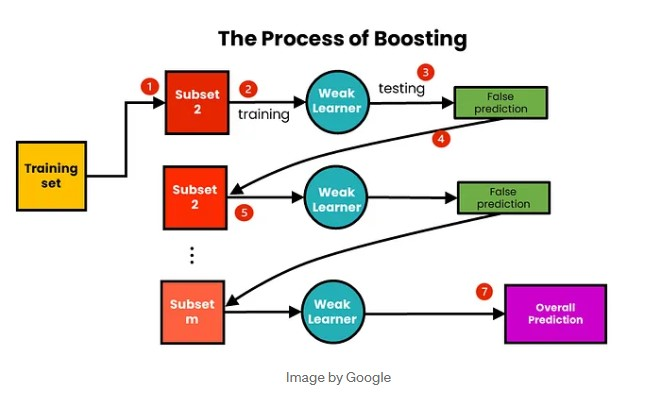
\includegraphics[width=0.6\textwidth]{Boosting.jpg}
\end{center}
\vspace{-0.2cm}
\footnotesize{Each weak learner learn from the mistakes of the previous learners leading to a more accurate and robust final model}
\end{frame}

\begin{frame}{Chosen Method: LightGBM}
\textbf{LightGBM Overview:}
\begin{itemize}
    \item Utilizes a histogram-based approach for faster training.
    \item Grows trees leaf-wise, which helps minimize loss more effectively.
\end{itemize}
\vspace{0.02cm} % Adds some spacing for better readability
\textbf{Histogram-based Approach:}
\begin{center}
    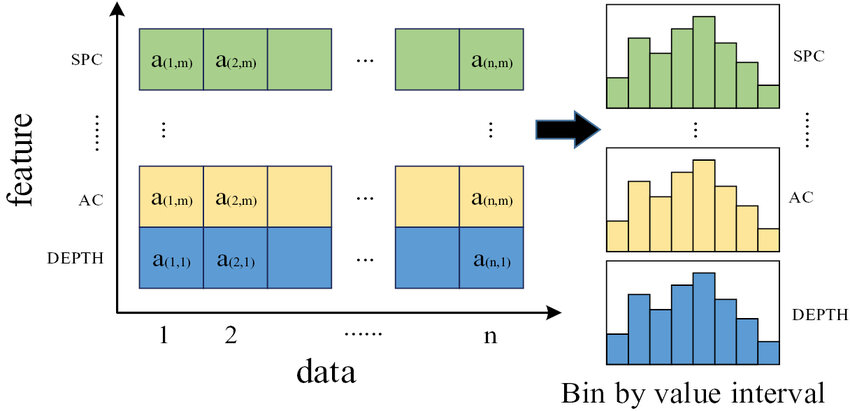
\includegraphics[width=0.38\textwidth]{HistBased.png}
\end{center}
\vspace{-0.2cm} % Adds spacing between sections
\textbf{Leaf-wise Tree Growth:}
\begin{center}
    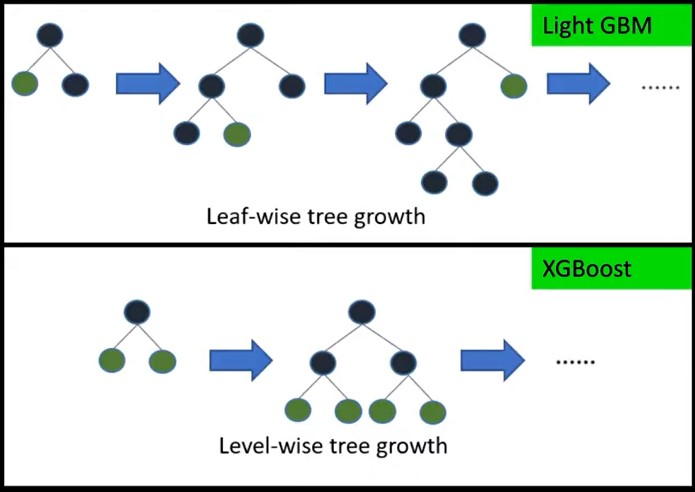
\includegraphics[width=0.35\textwidth]{Light.jpg}
\end{center}
\end{frame}

\begin{frame}{LightGBM: How It Works}
\textbf{Step-by-Step Process:}
\begin{itemize}
    \item Starts with a single decision tree predicting the target variable based on input features.
    \item Iteratively adds more decision trees, each correcting the errors of the previous tree.
\end{itemize}

\vspace{0.5cm} % Adds spacing for better visual separation

\textbf{Key Features of LightGBM:}
\begin{itemize}
    \item \textbf{Decision Tree Learning:} Forms the backbone of the algorithm.
    \item \textbf{Histogram-Based Approach:} Accelerates the training process by binning continuous data.
    \item \textbf{Leaf-Wise Tree Growth:} Minimizes loss more effectively than level-wise growth.
    \item \textbf{Regularization:} Prevents overfitting and improves model generalization.
\end{itemize}
\end{frame}

\begin{frame}{General Workflow of LightGBM}
\begin{center}
    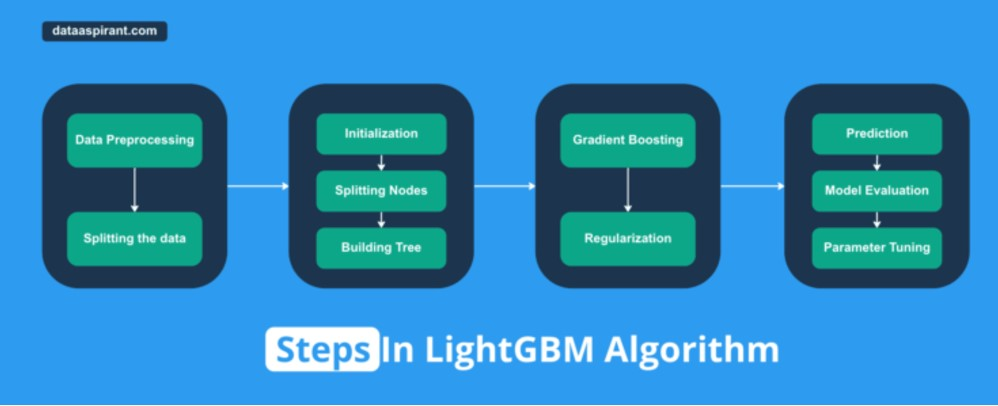
\includegraphics[width=0.9\textwidth]{Steps.jpg}
\end{center}
\end{frame}


% Section: Model Evaluation
\section{Model Evaluation}

\begin{frame}{Model Evaluation}
\textbf{Metrics:}
\begin{itemize}
    \item RMSE, MAE: Measure prediction accuracy.
    \item Poisson log-likelihood: Validates count data assumptions.
    \item R-squared: Goodness-of-fit.
\end{itemize}

\textbf{Validation Approach:}
\begin{itemize}
    \item Train-Valid split (80-20).
    \item Early stopping to avoid overfitting.
\end{itemize}

\textbf{Feature Importance:}
\begin{itemize}
    \item LightGBM's feature importance analysis to identify influential predictors.
\end{itemize}

\end{frame}

\begin{frame}{Hyperparameter Optimization: Steps Performed}
\textbf{Parameter Grid:}
\begin{itemize}
    \item Key Parameters: \texttt{num\_leaves}, \texttt{learning\_rate}, \texttt{feature\_fraction}, \texttt{min\_data\_in\_leaf}, \texttt{max\_depth}.
\end{itemize}

\textbf{Cross-Validation:}
\begin{itemize}
    \item 5-fold cross-validation using \texttt{lgb.cv}.
    \item Evaluation metric: Poisson loss.
    \item Early Stopping: Halted training if no improvement was observed within 50 rounds.
\end{itemize}

\textbf{Selection of Best Parameters:}
\begin{itemize}
    \item Tracked the lowest cross-validation score to select optimal parameters.
\end{itemize}
\end{frame}

\begin{frame}{Results: Best Parameters Identified}
\textbf{Optimal Parameters:}
\begin{itemize}
    \item \texttt{num\_leaves:} 127
    \item \texttt{learning\_rate:} 0.1
    \item \texttt{feature\_fraction:} 0.9
    \item \texttt{min\_data\_in\_leaf:} 100
    \item \texttt{max\_depth:} 5
\end{itemize}

\textbf{Training Performance Metrics}
\begin{itemize}
    \item \texttt{RMSE:} 35.68386
    \item \texttt{MAE:} 27.53179
    \item \texttt{Poisson Log-Loss:} 61.21314
    \item \texttt{R²:} 0.1124
\end{itemize}
\end{frame}

\begin{frame}{Feature Importance: Top Contributing Variables}
\textbf{Visualization:}
\begin{center}
    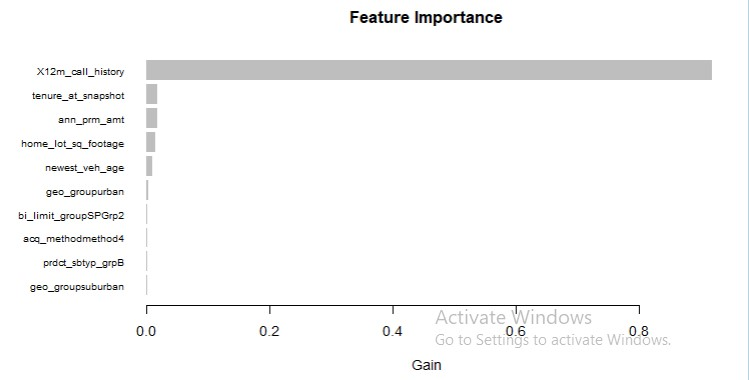
\includegraphics[width=0.8\textwidth]{Feature.jpg} 
\end{center}

\end{frame}


% Slide: Additional Variables
\begin{frame}{Potentially Useful Variables}
\textbf{Demographic Factors:}
\begin{itemize}
    \item Education level, marital status, employment status.
\end{itemize}

\textbf{Customer Behavioral Indicators:}
\begin{itemize}
    \item Payment history and risk profile, Duration of loyalty with the company, Frequency of customer service interactions.
\end{itemize}

\textbf{Policy and Service Features:}
\begin{itemize}
    \item Insurance add-ons or optional coverages, Payment frequency (e.g., monthly or annually), Policyholder location.
\end{itemize}

\end{frame}


% Section: Conclusion
\section{Conclusion}

\begin{frame}{Conclusion}
\textbf{Summary:}
\begin{itemize}
    \item LightGBM was selected for its efficiency, accuracy, and suitability for count data.
    \item Key predictors such as Past one year call count, Policy active length in month, Annualized Premium Amount, Square footage of the policyholder’s home lot, age of the newest vehicle insured on a policy were instrumental in explaining call counts.
    \item Model evaluation metrics confirmed the robustness of the approach.
\end{itemize}

\textbf{Future Work:}
\begin{itemize}
    \item Explore hyperparameter optimization (e.g., grid search).
    \item Incorporate other predictive features.
\end{itemize}
\end{frame}

\end{document}
